\section*{Abstract}


\section{Introduction}
\label{sec:intro}

Coastal zones provide the interface between the terrestrial domain and
the large expanse of the ocean which cover over 70\% of the surface of
the Earth. The transition between land and the ocean allows a range of
activities that make this domain critical for human wellbeing; from
trade, to tourism and sport, to its impact on food security for
sustainance based fishing communities as well as on national and
homeland security for facilities. With more than 600 Million people
living within 10 km of a coastline in the world, the impact of the
changing oceans has a disproportionate effect on a large area and
populations. 

While our understanding of such coastal environments have improved by
increased measurements of key variables especially sea surface height
(SSH), sea surface temperature (SST), tides, and pressure, all of
which have allowed for increased predictive power of oceanographic
events such as tsunamis, coastal surges, harmful algal blooms, hypoxia
(oxygen depletion), oil spills and coastal pollution. Modeling the
coastal zone with higher resolution and predictive power, has been
notoriously difficult given the distinct lack of scientific knowledge
we have of these highly mixed regions. The interaction of bathymetry,
physical forcings, riverine/estuarine interactions with the mixed surf
zone with strong tidal influences, implies that predictive
capabilities especially for loading/retrieving warfighters and assets,
are hamstrung by limited knowledge. The non-linearity of air/sea/land
interactions, the infusion of fresh water from riverine sources, the
proximity of anthropgenic sources of pollution in addition to the
nominal complexity of hydro-dynamic flow add to the challenges in
observing, measuring and predicting the state of any coastal
zone. Another principal challenge is gathering data in a synoptic as
well as systematic manner, across cohesive spatial and temporal scales
which can aid in the understanding of bio-geophysical
processes. Amalgamating, integrating and assimilating such data across
a range of critical ocean variables then, becomes a principal
technical task that to date have been difficult. With the onset of the
robotics and sensor technology revolution over the past decade, along
with the onset of explosion in work in both Machine Learning and
Artificial Intelligence methodologies, some of these challenges can
now be addressed.

Over the last decade a range of efforts primarily at universities in
the US, Europe and Australia have led to the development of low-cost
marine robotic platforms. These have benefited from incremental
developments in autonomous low-level control \cite{} as well as in
hardware subsystems and payloads related to measuring some of the
essential variables. Key variables in the ocean are often not directly
measurable; however sensing technology exists which can be a
proxy. Coupled with smaller form factor and optimized energy use and
leveraging battery technologies, these platforms have had extended use
in the aerial, surface and underwater domains. For instance, one
popular low-cost autonomous underwater vehicle (AUVs) now has the
capability to be on station for 5 days
\cite{sousa2012lauv,pinto2013lsts}. Small unmanned aerial vehicles
(UAVs) have had increased use in the battle space on land; however
those same technologies have proven to be equally useful over the
water, both as fixed wing as well as rotary platforms. Autonomous
surface vehicles (ASVs) however have made the biggest strides despite
being in the harsh surface environment, in part because they have been
able to capitalize on renewable sources of energy (wind, waves and
solar) to become persistent long-range assets for dual use
capabilities \cite{}.

\begin{figure}[!t]
  \centering
  \includegraphics[width=0.7\textwidth]{fig/Meteor-Fig-1.jpg}
  \caption{A multi-domain observation system which combines elements
    of hardware and software, onboard and on-shore, can provide
    high-resolution data in complex coastal conditions.}
  \label{fig:concept}
\end{figure}


Ocean models are non-linear software models which typically assimilate
data and make predictions on ocean physical (e.g. wind, waves,
turbulence, tides etc), thermal and bio-geochemical processes, driven
by bathymetry and coastal topography. Their forecasts, nowcasts and
hindcasts allow for predictions of oceanographic conditions from the
surface to the benthic environment. While these predictions are
approximations of real-world conditions, depending on the scale of the
prediction especially global or basin-scale, they provide reasonable
measures of predicibility for events; that is they're a major tool in
'ocean weather'. Recent advances in modeling have increased model
skill sufficiently that the notion of a 'digital twin' is being
frequently used for such models. However, the models continue to be
\emph{estimates} of reality; one approach to making predictions
converge to reality is via data assimilation especially from surface
remote sensing measurements. More recently, near real-time data from
buoys, drifters and even robots in-situ (Fig. \ref{fig:concept}) have
provided fine-scale data to ground models. As a result, it is
increasingly critical to use in-situ data and fast prediction
capability to test divergence between prediction and the ground
truth. Equally newer statistical methods \cite{lermusiaux06} within
the modeling framework are able to generate measures of coherance and
uncertainty, which can be quantified to direct more (or less) in-situ
data collection to \emph{reduce} such divergence between prediction
and the ground-truth.

Finally, the advent of Small Satellite platforms initially built by
students for single purpose uses, have prolifirated with significant
advances in payloads, control and propulsion leading to their adoption
commercially for a range of earth observing capabilities including for
ocean observation \cite{guerra16}. While individual satellites with
low-cost sensors can be assembled inexpensively (in the 100's of
thousands of dollars), the bottleneck of launch costs (in the
millions) are only now rapidly coming down with a number of US
domestic as well as international providing launch services with a
range of orbital orientations. This is driven in part because of
standardization allows launch providers to package large number of
\smle's (the largest to date has been 120) to lower unit costs, that
envisioning a private orbital constellation is now well within
reality. Some critical advantages of \smle's are that they can be
assembled quickly with the latest in optical or radar payloads,
integrated by small teams even within university environments, and
with lowered costs, can enable rapid revisit times with an orbital
``train'' of space-based sensors.

\begin{figure}[!]
  \centering
  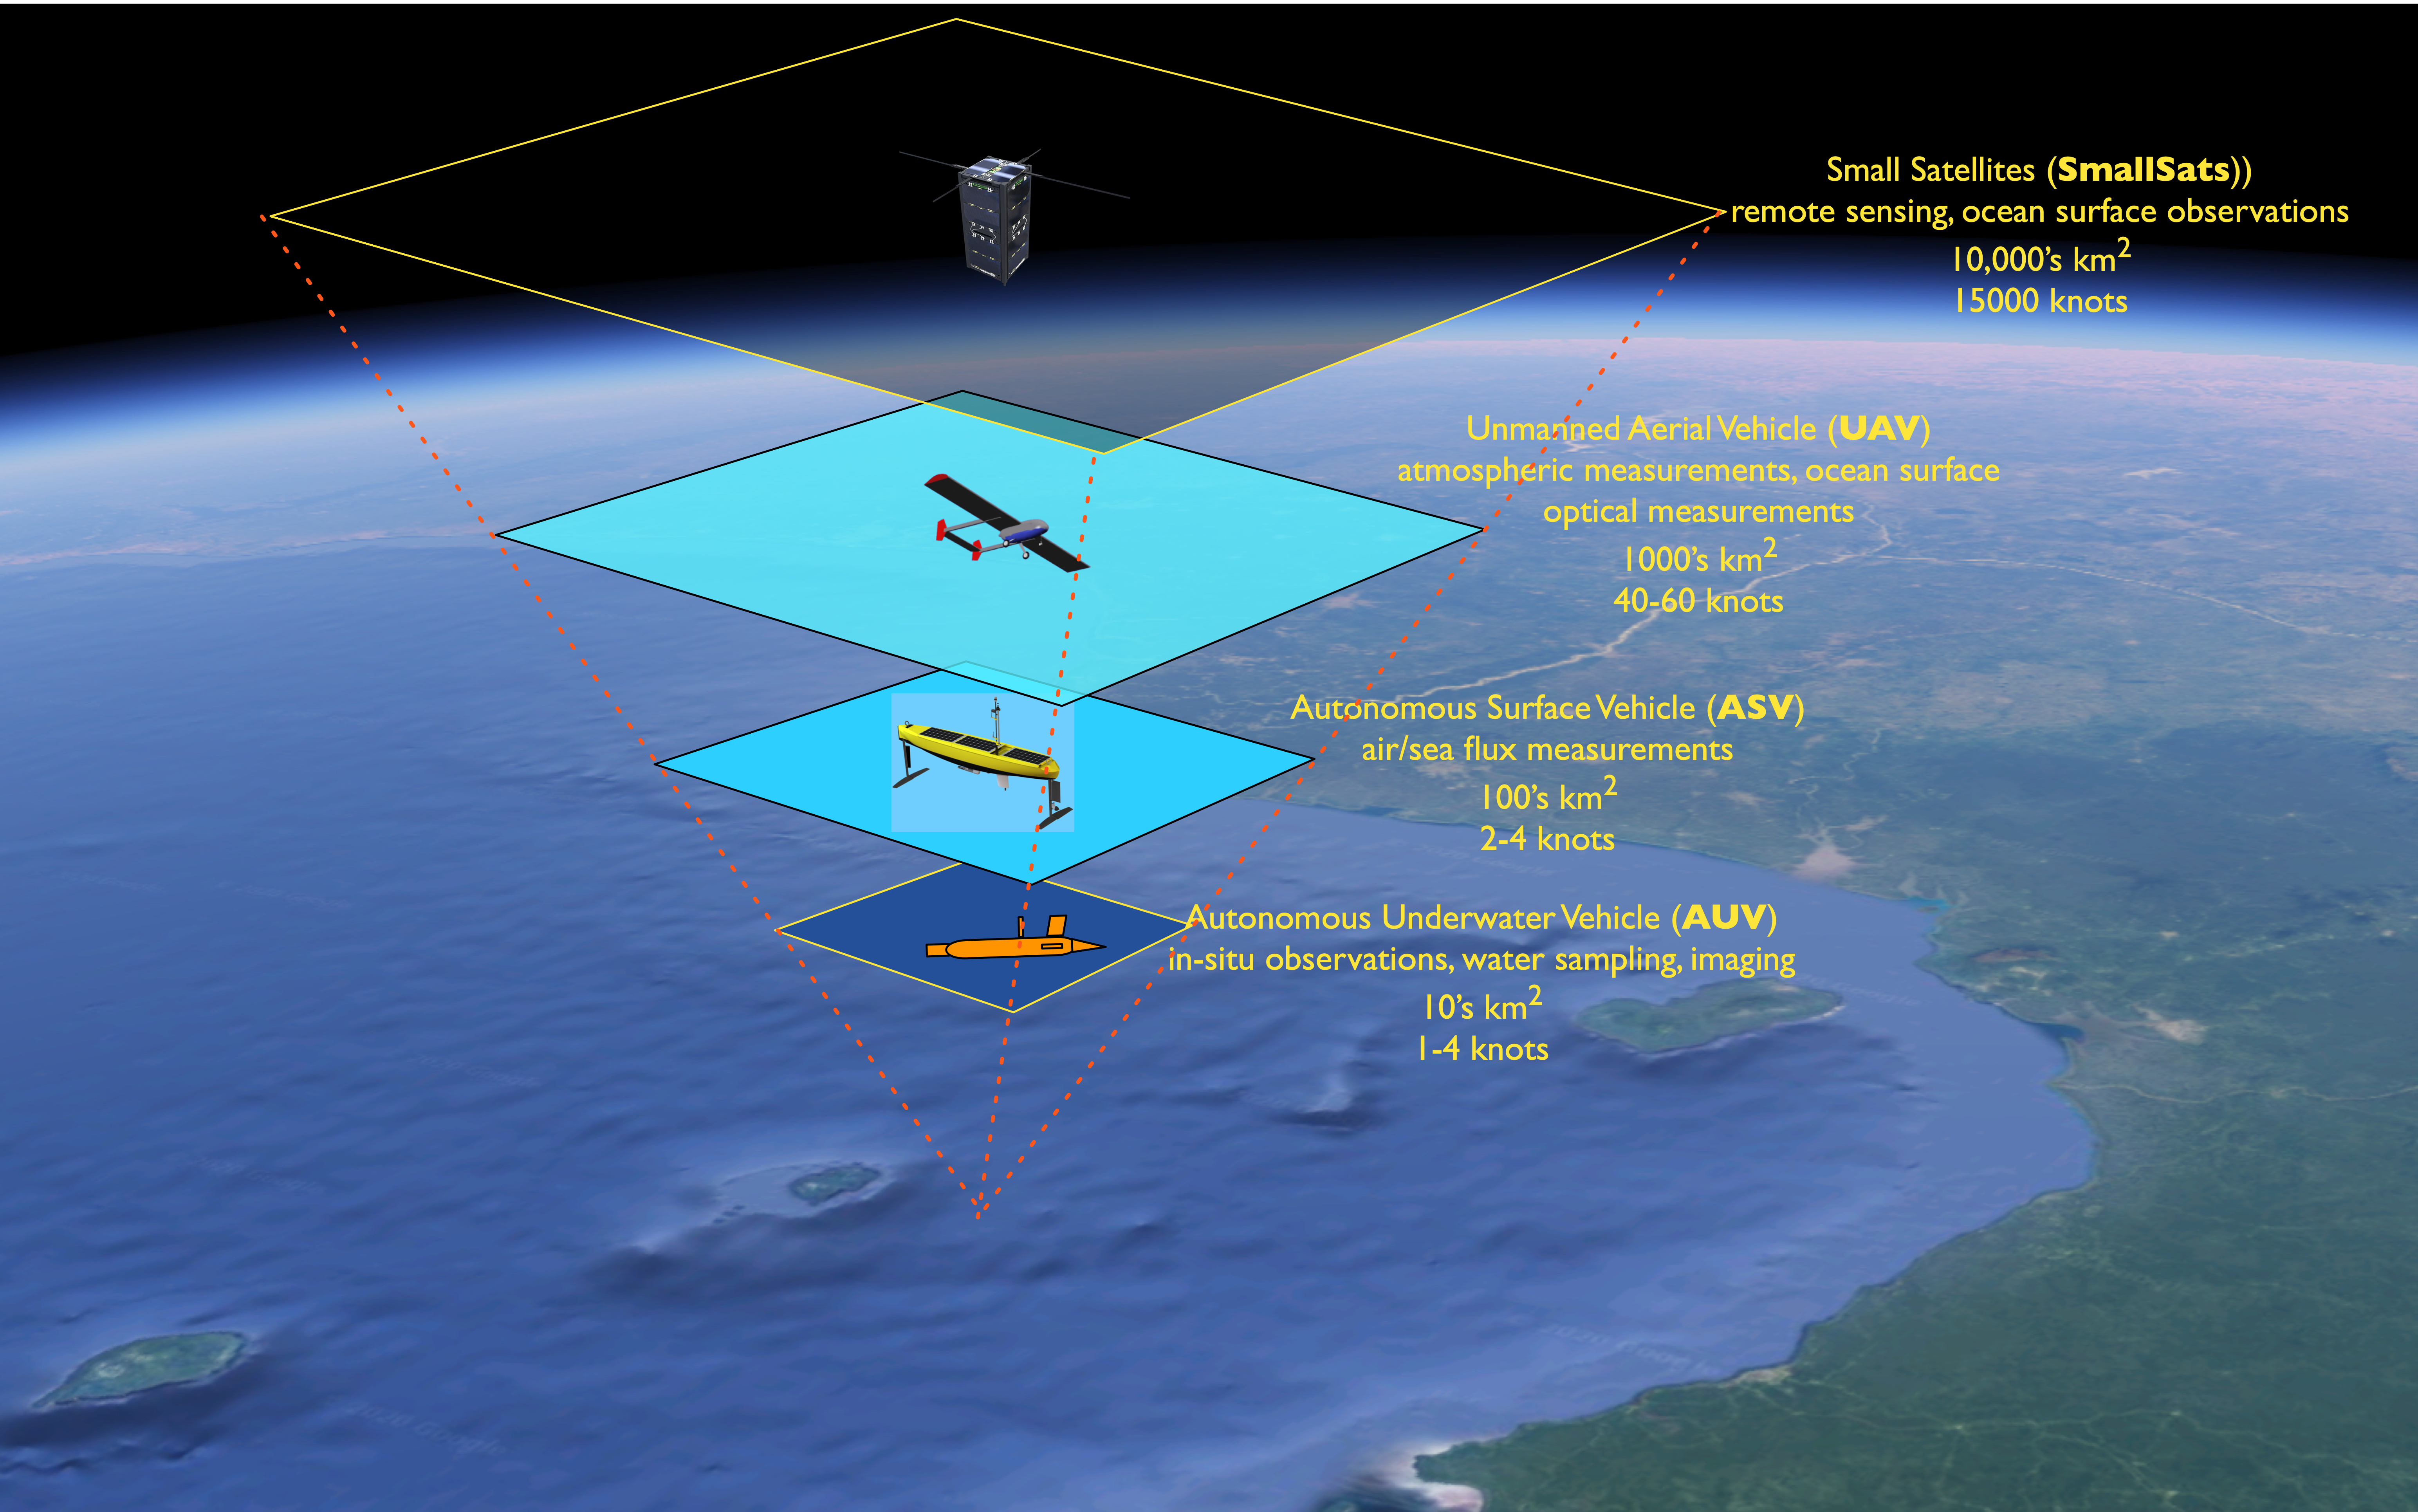
\includegraphics[width=1\textwidth]{fig/Meteor-Fig-3.jpg}
  \caption{An 'inverse pyramid' concept of observational tools using a
    mix of space, aerial, surface and underwater robots, observing a
    patch of the ocean.}
  \label{fig:concept-2}
\end{figure}


Combining these elements together by integrating agile low‐cost \sml
platforms, coupled with aerial, surface and underwater mobile and
immobile platforms we can now envision an observation system that
could provide low cost high‐resolution data at scales which are yet to
be realized. With high-revisit times, with \smle's carrying novel
technologies only a few years in the making (as against decades for
legacy agency based satellites), dynamic oceanographic events of
importance for civil and military needs can then be tracked. Equally,
and critically, with models run in the cloud, the entire ensemble is
portable and can be targeted to run in any coastal environment
(Fig. \ref{fig:concept-2}).

To enable this vision, however, we need to understand the principles
behind which such an observing system can be deployed and
operated. The remainder of this paper lays out this concept in some
detail; Section \ref{sec:related} reviews related work aligned with
this concept, Section \ref{sec:network} articulates and emphasiszes
the notion of networked elements for situational awareness, Section
\ref{sec:robots} explores the hardware elements including \smle's in
the ensemble, Section \ref{sec:decision} relates to intelligent
decision making within such an ensemble while Section
\ref{sec:applications} deals with dual-use applications. We conclude
with Section \ref{sec:wrapup} on ways to achieve such a distributed,
decision-theoretic concept and grounds it with how such a concept can
be realized. 